% -*- root: ../main.tex -*-
%!TEX root = ../main.tex
% this file is called up by main.tex
% content in this file will be fed into the main document
% vim:textwidth=80 fo=cqt

\clearpage
\chapter{Introduction}\label{ch:intro}

More introductory material goes here blah blah \dots \dots

This  thesis  strives to  represent  all  physical  quantities in  the  standard
International  System  of Units  (SI-Units).  However,  there are  some  notable
exceptions \eg{} for the capacity of a  Li-ion cell, which is represented in the
practical units of Ampere hours (\SI{}\amphours),  rather than the base SI Units
of Coulombs (\SI{}{\coulomb}). Such exceptions  are made taking into account the
prevalent conventions in standard literature.

\fxnote{make a note in the introduction  chapter that the terms cell and battery
are  used  interchangeably deviating  from  their  precise meaning,  \eg{}  cell
modelling and battery modelling}

% \cite{Grazioli2016a} goes crazy in reviewing the models out there.

% \cite{Seaman2014} provide a comprehensive survey  of the wide range of battery
% models out there.

Based on an isothermal description
Mention that stuff is applicable for both Lithium ion and Lithium polymer chemistries


\section{Chemistry}\label{subsec:liionchemistry}

This section  provides a  brief overview of  the essential  chemistry principles
that helps to provide a background context for the governing equations presented
in~\cref{subsec:basicspmgoverningeqns}.


In  a Li-ion  cell,  the  positive electrode  consists  of  porous particles  of
Lithium-Transition Metal Oxide (MO)  compounds. The negative electrode typically
employs  some  variant  of  microporous  graphite.  The  porous  nature  of  the
electrodes provide pathways for lithium  ion conduction through the electrolyte.
Due  to  the  special  construction  of the  electrode  structure,  there  exist
interstitial  sites  which act  as  intercalation  spots for  Lithium  shuttling
between the two  electrodes. The electrolyte, whose dynamics are  ignored in the
\gls{spm}, helps  in the  conduction of \ch{Li^+}  ions. The  separator membrane
allows  the passage  of  these ions  between the  two  electrodes, but  prevents
internal  short-circuit  by inhibiting  electronic  conduction  through it.  The
current collectors facilitate  passage of electrons generated  during the charge
transfer reaction  at particle surface  to the  external circuit. With  the help
of~\cref{fig:chargetransferprocess}  the  steps  involved  in  this  process  is
detailed next.

\begin{figure}[h]
    \centering
    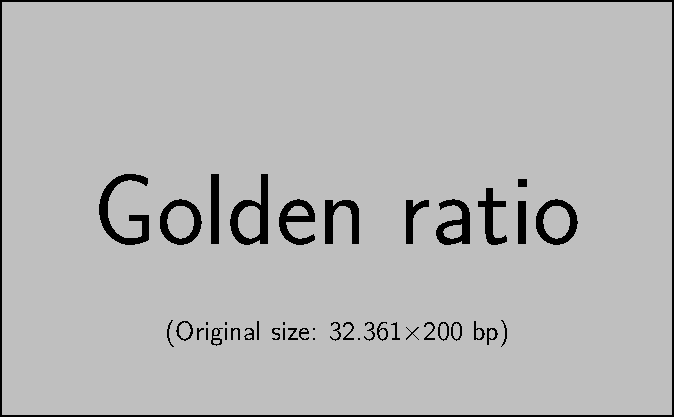
\includegraphics{placeholder_images/example-image-golden.pdf}
    \caption[Charge-transer and basic working mechanism of a Li-ion cell]{Simplified representation of charge-transfer
    process and illustration of basic working mechanism of a Li-ion cell.}
    \label{fig:chargetransferprocess}
\end{figure}

At fully  charged condition,  the majority  of Lithium in  the system  is stored
within  the  negative  electrode  microstructure.  During  discharge,  \ch{Li^0}
atoms  diffuse  out of  deep  interstitial  sites  towards  the surface  of  the
particles  in  the negative  electrode.  At  the surface  (electrode-electrolyte
interface),  a charge-transfer  process takes  place according  to Butler-Volmer
kinetics~\cref{eq:butlervolmer}, leading to the  formation of \ch{Li^+} ions and
electrons.  The electrons  are passed  to the  external circuit  through \ch{Cu}
current collectors  onto which  the conductive matrix  composed of  the negative
electrode material and binders is coated.  The \ch{Li^+} ions travel through the
electrolyte phase,  crossing the  separator membrane  to the  positive electrode
where they  encounter an  electron influx  from the  external circuit.  A charge
transfer  reaction  takes  place  at  the  surface  of  the  positive  electrode
particles, leading to the formation of neutral \ch{Li^0} atoms that diffuse into
the positive electrode microstructure.

During  the   charging  process,  the   reverse  phenomena  occur.   Lithium  is
de-intercalated  from  the  positive  electrode and  a  similar  charge-transfer
happens  at the  surface,  leading  to the  formation  of  \ch{Li^+} ions  which
reach  the  negative  electrode  by   passing  through  the  separator.  At  the
surface  of  the  negative  electrode particles,  these  ions  absorb  electrons
from  the  external circuit,  leading  to  the  formation of  neutral  \ch{Li^0}
that   diffuses  into   interior   vacant  spaces   in   the  layered   graphite
electrode. The  charge-transfer mechanism  and sequence  of events  are depicted
in~\cref{fig:chargetransferprocess}.
\Cref{eq:NegElectrodeRxn,eq:PosElectrodeRxn} summarise the reactions during the
charging and discharging process at the surfaces of both electrode materials.
\begin{align}
    \ch{Li_{$x$} C                            &<=>[\tiny{discharge}][\tiny{charge}] C + $x$ Li^+ + $x$ e^-}\label{eq:NegElectrodeRxn}\\
    \ch{Li_{1-$x$} M O2 + $x$ Li^+  + $x$ e^- &<=>[\tiny{discharge}][\tiny{charge}] LiMO2}\label{eq:PosElectrodeRxn}
\end{align}
where    \ch{M}   represents    a    transition   metal    compound   such    as
\ch{Ni_{1/3}Co_{1/3}Mn_{1/3}}   (NMC),   \ch{Ni_{0.8}Co_{0.15}Al_{0.05}}   (NCA)
amongst other  choices~\cite{Reddy2011}. Assuming  no loss of  cycleable Lithium
due to  parasitic side  reactions or  through other  mechanisms, the  process is
fully reversible.


The electrochemical potential at each electrode  is dependent upon the extent of
its  lithiation. An  empirical  relationship of  each  electrode's potential  as
a  function  of  its  stoichiometry  can be  obtained,  and  is  dependent  upon
the  specific design  and  material  properties of  each  active material  under
consideration. Finally, the \gls{ocv} of the cell is obtained by subtracting the
negative electrode potential from its positive electrode counterpart.

% -*- root: ../main.tex -*-
%!TEX root = ../main.tex
% this file is called up by main.tex
% content in this file will be fed into the main document
% vim:nospell textwidth=180 foldlevelstart=3 foldlevel=3

% \begin{table}[!htbp]
    \begin{table}[p]
        \centering
        \caption[]{}
        % \label{tbl:charSimspmp2d}
        \begin{threeparttable}
            \begingroup
            \makeatletter\def\f@size{10.0625}\check@mathfonts
            % \addtolength{\jot}{0.75em}
            \addtolength{\jot}{0.875em}
            \begin{tabular*}{\textwidth}{@{} l c r l r @{}}
                \toprule
                Region & Governing equations & \multicolumn{3}{c}{Boundary conditions} \\
                \midrule
                \multicolumn{1}{l |}{\rotatebox[origin=c]{+90}{\makecell{\small Electrodes \\ \small \linnegpos}}} &
                $\begin{aligned} % placement: default is "center", options are "top" and "bottom"
                    \vphantom{\diffp{c_\slsub}{r}{\mathrlap{r = R_\pl}}}
                    \diffp{c_\slsub}{t} &= \frac{D_\slsub}{r^2}\diffp{}{r}\left(r^2 \diffp{c_\slsub}{r} \right) \\
                    \vphantom{\diffp{c_\text{e}}{x}{\mathrlap{x = l_\text{tot}}}}
                    \varepsilon_l \diffp{c_\text{e}}{t} &= \diffp{}{x}\left(D_\effl
                    \diffp{c_\text{e}}{x} \right) + (1 - t^0_\text{+}) a_\slsub j_l \\
                    \vphantom{\diffp{\phi_\text{e}}{x}{\mathrlap{x = 0}}} 0 &= \diffp{}{x}\left(\kappa_\effl \diffp{\phi_\text{e}}{x}\right) + \diffp{}{x}\left(\kappa_\effl \frac{2 R T(t)}{F} (t^0_{+}-1)\diffp{ \ln c_\text{e}}{x}\right) \\
                    \vphantom{\sigma_\effl\!\diffp{\phi_\slsub}{x}{\mathrlap{\substack{\vphantom{\displaystyle M}x = x_\text{pos/sep}\\x = x_\text{neg/sep}}}}} a_\slsub F j_l &= \diffp{}{x}\left(\sigma_\effl \diffp{\phi_\slsub}{x}\right) \\
                    % j_l &= k_\lr c^\alpha_\text{e}\left(c_\slmax - c_\slsurf\right)^\alpha c^\alpha_\slsurf\left( \exp\left(\frac{\left(1-\alpha\right)F}{R T}\eta\right) - \exp\left(-\frac{\alpha F}{R T}\eta\right) \right)
                    j_l &= 2 k_\lr \sqrt{c_\text{e}\left(c_\slmax - c_\slsurf\right) c_\slsurf} \sinh \left(\frac{0.5 F}{R T(t)} \eta_l \right)
                \end{aligned}$ &
                $\begin{aligned}
                    \vphantom{\diffp{c_\slsub}{r}{\mathrlap{r = R_\pl}}} \diffp{c_\slsub}{r}{\mathrlap{r = 0}}\hspace{1mm} &= 0, \\
                    \vphantom{\diffp{c_\text{e}}{x}{\mathrlap{x = l_\text{tot}}}} \diffp{c_\text{e}}{x}{\mathrlap{x = 0}}\hspace{1mm} &= 0, \\
                    \diffp{\phi_\text{e}}{x}{\mathrlap{x = 0}}\hspace{1mm} &= 0, \\
                    \sigma_\effl\!\diffp{\phi_\slsub}{x}{\mathrlap{\substack{\vphantom{\displaystyle M}x = x_\text{pos/sep}\\x = x_\text{neg/sep}}}}\hspace{1mm} &= 0, \\
                    % {}&\textemdash{}{}
                    {}&\xdash[1.25em]{}
                \end{aligned}$ &
                $\begin{aligned}
                    \diffp{c_\slsub}{r}{\mathrlap{r = R_\pl}}\hspace{1mm} &= \frac{-j_l}{D_\slsub} \\
                    \diffp{c_\text{e}}{x}{\mathrlap{x = l_\text{tot}}}\hspace{1mm} &= 0 \\
                \vphantom{\diffp{\phi_\text{e}}{x}{\mathrlap{x = 0}}} \phi_\text{e}\Bigr\rvert_{\mathrlap{x=l_\text{tot}}} \hspace{1mm}&= 0 \\
                % \sigma_\effl\!\diffp{\phi_\slsub}{x}{\mathrlap{\subalign{x&=0\\x&=x_\text{tot}}}} &= \frac{-I}{A} \\
                \vphantom{\sigma_\effl\!\diffp{\phi_\slsub}{x}{\mathrlap{\substack{\vphantom{\displaystyle M}x = x_\text{pos/sep}\\x = x_\text{neg/sep}}}}} \sigma_\effl\!\diffp{\phi_\slsub}{x}{\mathrlap{\substack{\!\!\!\!\!x=0\\x=x_\text{tot}}}}\hspace{1mm} &= \frac{-I}{A} \\
                % \sigma_\effl\!\diffp{\phi_\slsub}{x}{\mathrlap{\substack{\begin{mysubarray} x &=0 \\ x &=x_\text{tot}\end{mysubarray}}}} &= \frac{-I}{A} \\
                % {}&\textemdash{}{}
                {}&\xdash[1.25em]{}
            \end{aligned}$ &
            $\begin{aligned}
                \vphantom{\diffp{c_\slsub}{r}{\mathrlap{r = R_\pl}}}\refstepcounter{equation}(\theequation)\label{eq:dfnsoliddiff} \\
                \vphantom{\diffp{c_\text{e}}{x}{\mathrlap{x = l_\text{tot}}}} \refstepcounter{equation}(\theequation)\label{eq:dfnliquiddiff} \\
                \vphantom{\diffp{\phi_\text{e}}{x}{\mathrlap{x = 0}}} \refstepcounter{equation}(\theequation) \\
                \vphantom{\sigma_\effl\!\diffp{\phi_\slsub}{x}{\mathrlap{\substack{\vphantom{\displaystyle M}x = x_\text{pos/sep}\\x = x_\text{neg/sep}}}}} \refstepcounter{equation}(\theequation) \\
                \vphantom{\left(\frac{0.5 F}{R T(t)} \eta \right)} \refstepcounter{equation}(\theequation)
            \end{aligned}$ \\
            \bottomrule
        \end{tabular*}
        \endgroup
        \begin{minipage}{\textwidth}
            \bigskip
            \begin{flushleft}
                \raggedright
                \makeatletter\def\f@size{14}\check@mathfonts
                $\begin{alignedat}{2}
                    & \text{\textbullet{} } c_\text{e} &  & \coloneqq c_\text{e}(x,t), \quad  \{x \in [0,l_\text{tot}],\, (x=0)\symbol{"2259} \text{\footnotesize pos/Alcc},\, (x=l_\text{tot})\symbol{"2259} \text{\footnotesize neg/Cucc}\}  \tnote{\dagger}                                                                                                                                                                  \\
                    & \text{\textbullet{} } \phi_\text{e} &  & \coloneqq \phi_\text{e}(x,t)\\
                \end{alignedat}$
                \\[0.5em]
                \fbox{\raggedright \small  \linnegpos}
                $\begin{alignedat}{2}
                    % & \mathbf{\textbf \linnegpos} & {} \\
                    & \text{\textbullet{} } c_\slsub   &  & \coloneqq c_\slsub(r,t), \quad  \{r \in [0,R_\pl],\, (r=0)\symbol{"2259} \text{\footnotesize  particle center},\, (r=R_\pl)\symbol{"2259} \text{\footnotesize particle surface}\}              \\
                    & \text{\textbullet{} } c_\slsurf &  & \coloneqq c_\slsub(r=R_\pl,t)\\
                    & \text{\textbullet{} } \phi_\slsub &  & \coloneqq \phi_\slsub(x,t)\\
                    & \text{\textbullet{} } j_l          &  & \coloneqq j_l(x,t) \\
                    & \text{\textbullet{} } \sigma_\effl &  & = \sigma_l \cdot \varepsilon_l \\
                    & \text{\textbullet{} } \eta_l        &  & \coloneqq \eta_l(x,t) = \phi_\slsub(x,t) - \phi_\text{e}(x,t) - \mathcal{U}_l(c_\slsurf) \\[0.5em]
                \end{alignedat}$
                % \medskip
                \fbox{\raggedright \small  \linnegseppos}\\[0.5ex]
                $\begin{alignedat}{2}
                    & \text{\textbullet{} } D_\effl    &  & = D \cdot \varepsilon_l^{\text{brugg}_l}                                                                                                                                                  \\
                    & \text{\textbullet{} } \kappa_\effl &  & = \kappa \cdot \varepsilon_l^{\text{brugg}_l} \\
                    & \text{\textbullet{} } D        &  & \coloneqq D(c_\text{e},T) = 10^{-4} \times 10^{-4.43 - \frac{54}{T(t) - 229 - 5\times10^{-3} c_\text{e}(x,t)} - 0.22\times10^{-3} c_\text{e}(x,t)}               \\
                \end{alignedat}$
                \\
                \makeatletter\def\f@size{14}\check@mathfonts
                $\begin{alignedat}{2}
                    & \text{\textbullet{} }  \kappa   \: \quad&  & \coloneqq \kappa(c_\text{e},T)\, = \parbox[t]{11.60cm}{\raggedright $\scriptstyle 10^{-4} \times c_\text{e}(x,t)\Big(-10.5 + 0.668\times10^{-3} c_\text{e}(x,t) + 0.494\times10^{-6} c_\text{e}^2(x,t) + \big(0.074 - 1.78\times10^{-5}c_\text{e}(x,t) - 8.86\times10^{-10}c_\text{e}^2(x,t)\big)T(t) + \big(-6.96\times10^{-5} + 2.8\times10^{-8} c_\text{e}(x,t)\big)T^2(t)\Big)^2$}\\
                \end{alignedat}$
            \end{flushleft}
        \end{minipage}
        \bigskip
        \footnoterule{}
        \begin{tablenotes}
        \item[\dagger] \footnotesize{This definition of the global axial domain $x$, spanning the cell thickness applies for all variables dependent on axial spatial position. Hence the domain definition for $x$ is not repeated elsewhere for the sake of brevity.}
        \end{tablenotes}
    \end{threeparttable}
\end{table}


% write about lumped thermal model equations here. Point out to relevant
% parameters
